\documentclass[aspectratio=169,11pt]{beamer}
\usetheme{Warsaw}
\usepackage[utf8]{inputenc}
\usepackage[polish]{babel}
\usepackage{amsmath}
\usepackage{amsfonts}
\usepackage{amssymb}
\usepackage{graphicx}
\author{Marcin Skrzypkowski}
\title{Autonomiczna nawigacja manipulatora mobilnego}

%\setbeamercovered{transparent} 
%\setbeamertemplate{navigation symbols}{} 
%\logo{} 
%\institute{} 
%\date{} 
%\subject{} 

\usepackage[
    backend=bibtex,
    style=ieee
]{biblatex}

\addbibresource{sources.bib}

%set page counters
\addtobeamertemplate{navigation symbols}{}{%
    \usebeamerfont{footline}%
    \usebeamercolor[fg]{footline}%
    \hspace{1cm}%
    \insertframenumber/\inserttotalframenumber
}

%remove navigation bar from slide
%\AtBeginSection[] % Do nothing for \section*
%{
%\begingroup
%\setbeamertemplate{headline}{}
%%\addtobeamertemplate{frametitle}{\vspace*{-1\baselineskip}}{}
%\addtobeamertemplate{frametitle}{\vspace*{-1cm}}{}
%\begin{frame}<beamer>
%\frametitle{Title}
%%\tableofcontents[currentsection]
%\end{frame}
%\endgroup
%}


%define new subsection for display in frames
\setbeamercovered{transparent}

\makeatletter
\let\oldheadcommand\headcommand
\newcommand{\stopnavigation}{\addtocontents{nav}{\string\let\string\headcommand\string\@gobble}}
\newcommand{\resumenavigation}{\addtocontents{nav}{\string\let\string\headcommand\string\oldheadcommand}}


%\newcount\c@p
%\newcount\c@m
%\def\insertsectionnavigation#1{%
%  \hbox to #1{%
%    \vbox{{\usebeamerfont{section in head/foot}\usebeamercolor[fg]{section in head/foot}%
%     \vskip0.5625ex%
%    \def\slideentry##1##2##3##4##5##6{}%
%     \def\sectionentry##1##2##3##4##5{%
%       \ifnum##5=\c@part%
%       \def\insertsectionhead{##2}%
%       \def\insertsectionheadnumber{##1}%
%       \def\insertpartheadnumber{##5}%
%       \c@p=\c@section%
%       \c@m=\c@section%
%       \advance\c@m by -1 %
%       \advance\c@p by 1 %
%             \ifnum\c@section=##1%
%               \setbox\beamer@tempbox=\hbox{%
%              \hyperlink{Navigation##3}{\hbox to #1{%
%             {\hskip0.3cm\usebeamertemplate{section in head/foot}\hskip0.3cm}}}}%
%             \else%
%                 \ifnum##1=\c@m%
%                 \setbox\beamer@tempbox=\hbox{%
%                  \hyperlink{Navigation##3}{\hbox to #1{%
%                 {\hskip0.3cm\usebeamertemplate{section in head/foot shaded}\hskip0.3cm}}}}
%                 %
%                \else%
%                 \ifnum##1=\c@p%
%                 \setbox\beamer@tempbox=\hbox{%
%                  \hyperlink{Navigation##3}{\hbox to #1{%
%               {\hskip0.3cm\usebeamertemplate{section in head/foot shaded}\hskip0.3cm}}}}%
%               %
%               \else%
%               %
%               \fi%
%               \fi%
%               %
%            \fi%%
%            %
%
%      \ht\beamer@tempbox=1.6875ex%
%       \dp\beamer@tempbox=0.75ex%
%       \box\beamer@tempbox\fi}%
%     \dohead\vskip0.5625ex}}\hfil}}
%
%
%\setbeamertemplate{headline}%{split theme} % full manual adjustment
%{%
%  \leavevmode%
%  \@tempdimb=3em%
%  \ifdim\@tempdimb>0pt%
%    \advance\@tempdimb by 1.825ex%
%    \begin{beamercolorbox}[wd=.5\paperwidth,ht=\@tempdimb]{section in head/foot}%
%      \vbox to\@tempdimb{\vfil\insertsectionnavigation{.5\paperwidth}\vfil}%
%    \end{beamercolorbox}%
%    \begin{beamercolorbox}[wd=.5\paperwidth,ht=\@tempdimb]{subsection in head/foot}%
%      \vbox to\@tempdimb{\vfil\insertsubsectionnavigation{.5\paperwidth}\vfil}%
%    \end{beamercolorbox}%
%  \fi%
%}
%
%
%
%\makeatother




\newcounter{prevsection}
\newcounter{nextsection}

\newcommand\prevsection{}
\newcommand\nextsection{}

\makeatletter
\long\def\beamer@section[#1]#2{%
  \beamer@savemode%
    \mode<all>%
  \ifbeamer@inlecture%
   \refstepcounter{section}%
    \beamer@ifempty{#2}%
    {\long\def\secname{#1}\long\def\lastsection{#1}}%
    {\global\advance\beamer@tocsectionnumber by 1\relax%
      \long\def\secname{#2}%
      \long\def\lastsection{#1}%
      \addtocontents{toc}{\protect\beamer@sectionintoc{\the\c@section}{#2}{\the\c@page}{\the\c@part}%
        {\the\beamer@tocsectionnumber}}}%
    {\let\\=\relax\xdef\sectionlink{{Navigation\the\c@page}{\noexpand\secname}}}%
    \beamer@tempcount=\c@page\advance\beamer@tempcount by -1%
    \beamer@ifempty{#1}{}{%
      \addtocontents{nav}{\protect\headcommand{\protect\sectionentry{\the\c@section}{#1}{\the\c@page}{\secname}{\the\c@part}}}%
      \addtocontents{nav}{\protect\headcommand{\protect\beamer@sectionpages{\the\beamer@sectionstartpage}{\the\beamer@tempcount}}}%
      \addtocontents{nav}{\protect\headcommand{\protect\beamer@subsectionpages{\the\beamer@subsectionstartpage}{\the\beamer@tempcount}}}%
    }%
    \beamer@sectionstartpage=\c@page%
    \beamer@subsectionstartpage=\c@page%
    \def\insertsection{\expandafter\hyperlink\sectionlink}%
    \def\insertsubsection{}%
    \def\insertsubsubsection{}%
    \def\insertsectionhead{\hyperlink{Navigation\the\c@page}{#1}}%
    \def\insertsubsectionhead{}%
    \def\insertsubsubsectionhead{}%
    \def\lastsubsection{}%
    \Hy@writebookmark{\the\c@section}{\secname}{Outline\the\c@part.\the\c@section}{2}{toc}%
    \hyper@anchorstart{Outline\the\c@part.\the\c@section}\hyper@anchorend%
    \beamer@ifempty{#2}{\beamer@atbeginsections}{\beamer@atbeginsection}%
  \fi%
  \beamer@resumemode
    \setcounter{prevsection}{\thesection}%
    \setcounter{nextsection}{\thesection}%
    \addtocounter{prevsection}{-1}%
    \gdef\prevsection{\csname section\romannumeral\theprevsection \endcsname}%
     \addtocounter{nextsection}{1}%
    \renewcommand\nextsection{\csname section\romannumeral\thenextsection \endcsname}%
}%

\setbeamertemplate{headline}
{%
  \leavevmode%
  \@tempdimb=1.2ex%
  \ifnum\beamer@subsectionmax<\beamer@sectionmax%
    \multiply\@tempdimb by\beamer@sectionmax%
  \else%
    \multiply\@tempdimb by\beamer@subsectionmax%
  \fi%
  \ifdim\@tempdimb>0pt%
    \advance\@tempdimb by 1.125ex%
    \begin{beamercolorbox}[wd=.5\paperwidth,ht=\@tempdimb,right,rightskip=1em]{section in head/foot}%
      \vbox to \@tempdimb{%
      \ifnum\thesection=1 \else%
        \vfill{\color{fg!40!bg}\prevsection}%
      \fi%
        \vfill\insertsectionhead%
      \ifnum\thesection=\beamer@sectionmax \else%
        \vfill{\color{fg!40!bg}\nextsection}%
     \fi\vfill%
    }%
    \end{beamercolorbox}%
    \begin{beamercolorbox}[wd=.5\paperwidth,ht=\@tempdimb]{subsection in head/foot}%
      \vbox to\@tempdimb{\vfil\insertsubsectionnavigation{.5\paperwidth}\vfil}%
    \end{beamercolorbox}%
  \fi%
}%
\makeatother

% Here you put the names that will go in the navigation bar
\newcommand\sectioni{Robot Velma}
\newcommand\sectionii{Mapa}
\newcommand\sectioniii{Mapa kosztów}
\newcommand\sectioniv{Lokalizacja}
\newcommand\sectionv{Slam}
\newcommand\sectionvi{Planowanie ścieżki}
\newcommand\sectionvii{Navigation Stack}
\newcommand\sectionviii{Sformułowanie zadań}
\newcommand\sectionix{Dotychczasowe wyniki}
\newcommand\sectionx{Zadania do wykonania}
\newcommand\sectionxi{Zakończenie}


\begin{document}
{
\setbeamertemplate{headline}{}
\begin{frame}
\titlepage
	\begin{center}
		promotor: dr hab. inż. Wojciech Szynkiewicz
	\end{center}
\end{frame}
}

{
\setbeamertemplate{headline}{}
%\addtobeamertemplate{frametitle}{\vspace*{-1\baselineskip}}{}
\addtobeamertemplate{frametitle}{\vspace*{-2\baselineskip}}{}
\begin{frame}
\frametitle{Wstęp}
%	zdjęcie Velmy z labu i w symulacji
\end{frame}
}

{
\setbeamertemplate{headline}{}
\addtobeamertemplate{frametitle}{\vspace*{-2\baselineskip}}{}
\begin{frame}
\frametitle{Spis treści}
\tableofcontents
\end{frame}
}
%\stopnavigation


{
\setbeamertemplate{headline}{}
\addtobeamertemplate{frametitle}{\vspace*{-4\baselineskip}}{}
\begin{frame}
\frametitle{NAWIGACJA}
	\begin{center}
		\LARGE{\textbf{NAWIGACJA}}
	\end{center}
\end{frame}
}


\section{Robot Velma}

\begin{frame}{Symulacja robota}
%	zdjęcie Velmy w środowisku
	\begin{columns}
		\begin{column}{0.5\textwidth}
			\begin{itemize}
				\item Robot Velma - dwa manipulatory, każdy o siedmiu stopniach swobody
				
				
				\item Dostępne czujniki przydatne w nawigacji - dwa czujniki LiDAR, kamera Kinect, kamery RGB, jednostka inercyjna, czujniki odometrii (enkodery) na osiach kół bazy mobilnej (jedynie w rzeczywistym robocie, w symulacji odometria jest realizowana w inny sposób)
				
			\end{itemize}
		\end{column}
		\begin{column}{0.5\textwidth}
			\begin{itemize}
				
				\item Symulacja robota stworzona na potrzeby prac laboratoryjnych, w początkowych fazach projektów prace na samym robocie są zbyt niebezpieczne
				\item Baza mobilna - wielokierunkowa, wykorzystująca koła szwedzkie
			\end{itemize}
		\end{column}		
	\end{columns}
	
\end{frame}

\begin{frame}
\frametitle{Problemy z nawigacją robota Velma}
	\begin{itemize}
		\item należy wykrywać przeszkody znajdujące się wysoko ponad poziomem podłogi
		\item należy dobrać odpowiedni algorytm planowania i wykonania ścieżki wykorzystujący w pełni możliwości wielokierunkowej bazy mobilnej
		\item z powodu relatywnie skomplikowanej zasady działania napędu bazy mobilnej uproszczona implementacja systemu napędowego, co zmienia sposób implementacji odometrii
	\end{itemize}
\end{frame}

\begin{frame}
{Wykorzystywane narzędzia}
	\begin{columns}
		\begin{column}{0.25\textwidth}
			\begin{figure}
				\begin{center}
					
\includegraphics[width=\textwidth]{img/Ros_logo.png}
				\end{center}
			\end{figure}
		\end{column}
		\begin{column}{0.25\textwidth}  %%<--- here
						\begin{figure}
				\begin{center}
					
\includegraphics[width=\textwidth]{img/Gazebo_logo.png}		
				\end{center}
			\end{figure}
		\end{column}
				\begin{column}{0.25\textwidth}
			\begin{figure}
				\begin{center}
					
\includegraphics[width=\textwidth]{img/Python_logo.png}			
				\end{center}
			\end{figure}
		\end{column}
		\begin{column}{0.25\textwidth}  %%<--- here
						\begin{figure}
				\begin{center}
					
\includegraphics[width=\textwidth]{img/C++_Logo.png}
				\end{center}
			\end{figure}
		\end{column}
	\end{columns}
\footnotesize{Żródła: wikipedia.org, pngkey.com}
\end{frame}

\begin{frame}{Oprogramowanie części mobilnej}
	\begin{columns}
		\begin{column}{0.5\textwidth}
			\begin{center}
				ROS
			\end{center}
			\begin{itemize}
				\item popularny i rozwijany system programowania robotów
				\item umożliwia tworzenie niezależnych procesów w systemie operacyjnym komputera
				\item komunikacja między procesami za pomocą jednokierunkowych tematów i dwukierunkowych serwisów
			\end{itemize}
			
		\end{column}
		\begin{column}{0.5\textwidth}  %%<--- here
			\begin{center}
				GAZEBO
			\end{center}
			\begin{itemize}
				\item symulowanie obiektów w przestrzeni trójwymiarowej
				\item proste pisanie własnych wtyczek w C++
				\item początkowo część ROSa, teraz niezależna platforma
			\end{itemize}
		\end{column}
	\end{columns}
\end{frame}


\begin{frame}{Symulacja części mobilnej}
	\begin{columns}
		\begin{column}{0.5\textwidth}
			\begin{center}
				MODUŁ SYMULACYJNY
			\end{center}
			\begin{itemize}
				\item definicja kształtu wizualnego obiektów
				\item definicja kolizji obiektów
				\item definicja dynamiki obiektów
			\end{itemize}
			
		\end{column}
		\begin{column}{0.5\textwidth}  %%<--- here
			\begin{center}
				MODUŁ STERUJĄCY BAZY JEZDNEJ
			\end{center}
			\begin{itemize}
				\item wykorzystuje informacje o parametrach kolizji i dynamiki z pierwszego modułu
				\item przyjmuje jako wejście prędkość zadaną bazy
				\item oblicza siły działające na bazę
			\end{itemize}
		\end{column}
	\end{columns}
\end{frame}



\section{Mapa}


\begin{frame}{Do czego potrzebna jest mapa}
	Możliwa jest nawigacja bez wykorzystania mapy, w tym wypadku wykorzystuje się tak zwaną nawigację zliczeniową. 
	Jej wykorzystanie powoduje akumulację błędu pozycji, którego nie da się zniwelować,
	a który rośnie z czasem.
	Dlatego potrzebne są punkty orientacyjne, które pozwalają utrzymać błąd lokalizacji w pewnych granicach.
	
%TODO	Robotics Vision and Control
\end{frame}

\begin{frame}{Jak działa budowa mapy}
	\begin{itemize}
		\item początkowe założenie - znana pierwotna pozycja robota
		\item uzyskanie punktów otoczenia względem robota
		\item możliwośc wykorzystania wielu czujników - systemu LiDAR, kamery Kinect, sonarów etc.
		\item możliwość identyfikowania poszczególnych punktów na mapie aby moć je od razu rozpoznać lub przechowywanie jedynie współrzędnych zajętych obszarów
	\end{itemize}
\end{frame}

\begin{frame}{Jak działa budowa mapy}
%TODO	zdjęcie budowy lidarem i kinectem
\end{frame}

\begin{frame}{Własności niektórych metod}
	\begin{columns}
		\begin{column}{0.5\textwidth}
			\begin{center}
				czujnik LiDAR
			\end{center}
			\begin{itemize}
				\item szybkie tworzenie obrazów dużych płaskich przestrzeni
				\item informacje pobrane tylko na jednej wysokości, zwykle blisko podłoża (mapa 2D)
			\end{itemize}
		\end{column}
		\begin{column}{0.5\textwidth}  %%<--- here
			\begin{center}
				kamera Kinect
			\end{center}
			\begin{itemize}
				\item mniejszy kąt widzenia czujnika i większe nakłady obliczeniowe - potrzeba więcej zasobów do budowy takiej mapy				
				\item budowa obrazu trójwymiarowej przestrzeni
			\end{itemize}
		\end{column}
	\end{columns}
\end{frame}


\section{Mapa kosztów}

\begin{frame}{Czym jest mapa kosztów}
	\begin{itemize}
		\item mapa - informacje które punkty w przestrzeni są zajęte, ewentualnie informacje o ich identyfikacji
		\item mapa kosztów - każdy punkt w przestrzeni ma przypisaną pewną wartość (binarnie lub z większym przedziałem), wykorzystywana w algorytmach wyszukiwania ścieżki
		\item przez dodawanie wartości pośrednich można sprawić by algorytm unikał nieporządanych miejsc jak pobliże ścian czy śliska nawierzchnia
	\end{itemize}
\end{frame}

\begin{frame}{Mapa i mapa kosztów}
\begin{columns}
		\begin{column}{0.5\textwidth}
			\begin{center}
				MAPA
				\begin{figure}
					\centering
					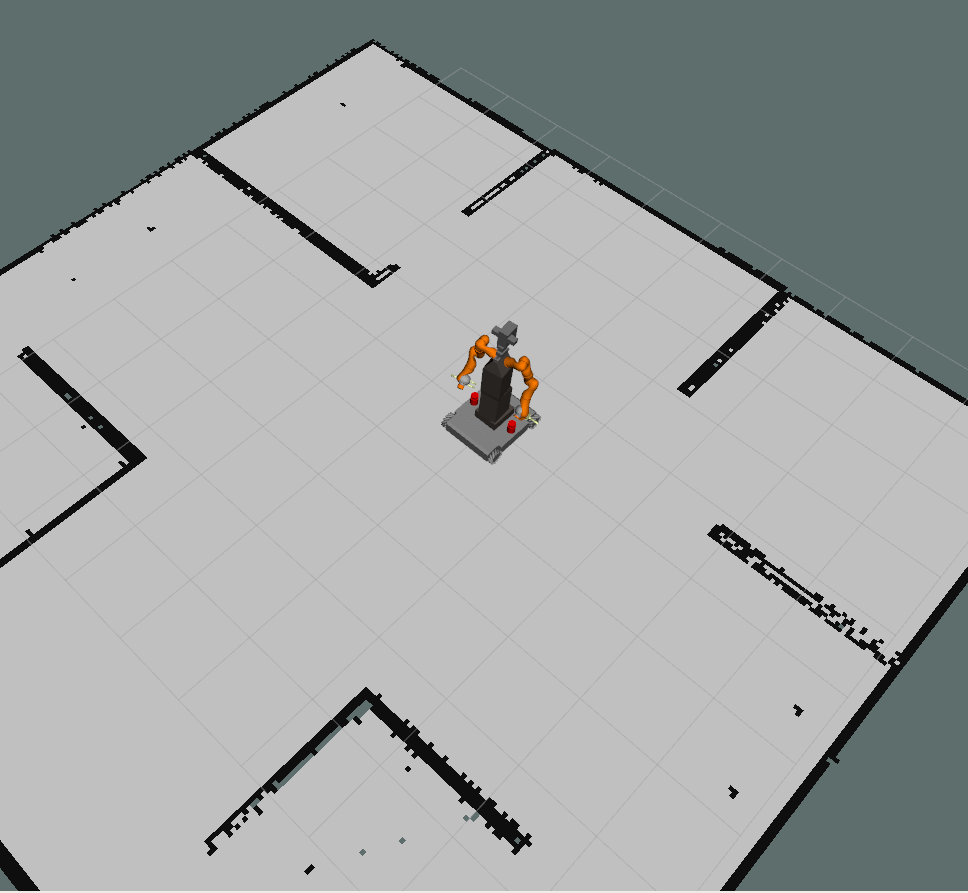
\includegraphics[height=0.55\textheight]{img/mapa_2d.png}
					\caption{dwuwymiarowa mapa środowiska}
				\end{figure}
			\end{center}
		\end{column}
		\begin{column}{0.5\textwidth}  %%<--- here
			\begin{center}
				MAPA KOSZTÓW
				\begin{figure}
					\centering
					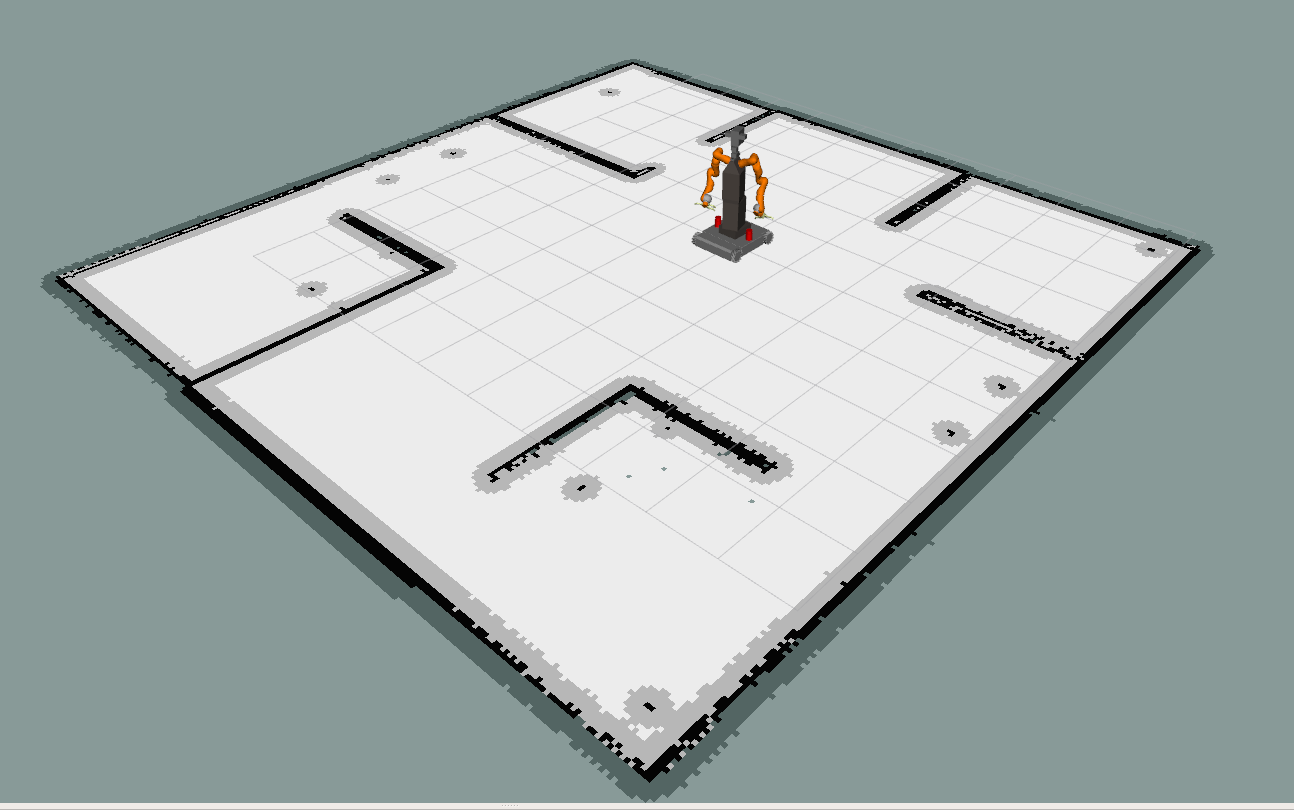
\includegraphics[height=0.55\textheight]{img/costmapa.png}
					\caption{jednowarstwowa mapa kosztów środowiska na podstawie mapy 2d}
				\end{figure}
			\end{center}
		\end{column}
	\end{columns}
\end{frame}

\begin{frame}
{Wielowarstwowe mapy kosztów}
\begin{columns}
		\begin{column}{0.5\textwidth}
			\begin{itemize}
				\item pozwalają na zobrazowanie kosztu poruszania w większej ilości kontekstów (ruch prawostronny, omijanie przestrzeni publicznej)
				\item możliwość wykrywania przeszkód na kilku poziomach (przykładowo wykrycie blatu stołu)
				\item możliwość wykorzystania chmury punktów z Kinecta do stworzenia mapy kosztów przez zrzutowanie wszystkich punktów na płaszczyznę
			\end{itemize}
		\end{column}
		\begin{column}{0.5\textwidth}  %%<--- here
			\begin{figure}
				\begin{center}
					\includegraphics[page={1},clip, trim=12.5cm 15cm 4cm 6cm, scale=0.6]{pdf/Layered_Costmaps_for_Context-Sensitive_Navigation-14.pdf}
					\hspace*{5pt}\hbox{\scriptsize{Źródło:\thinspace{\footnotesize{\itshape{David V. Lu, Dave Hershberger \cite{layered_costmap}}}}}}
					\caption{Przykład wielowarstwowej mapy kosztów }
				\end{center}
			\end{figure}
		\end{column}
	\end{columns}
\end{frame}



\section{Lokalizacja}

\begin{frame}
{Macierz przekształcenia jednorodnego}
Poniżej znajduje się jedna z interpretacji macierzy przekształcenia jednorodnego.
Przedstawia operację przejścia z układu współrzędnych $0$ do $1$. 
Dzięki temu można przekształcić pozycję obiektu znajdującego się w układzie $0$ i przedstawić jako pozycję względem układu $1$.
Dodatkowo można z niej odczytać położenie i orientację układu $1$ w układzie $0$.
\begin{equation*}
	\prescript{0}{1}T = 
	\begin{bmatrix}
		r_{}11 	& r_{}12	&	r_{}13	& \prescript{0}{1}P_x \\
		r_{}21 	& r_{}22	&	r_{}23	& \prescript{0}{1}P_y \\
		r_{}31 	& r_{}32	& r_{}33	& \prescript{0}{1}P_z \\
		0				&	0				&	0				&	1										\\
	\end{bmatrix}
	\Rightarrow
		\prescript{0}{1}T = 
	 \left[ \begin{array}{c|c}
   \prescript{0}{1}R_{3x3} 	& \prescript{0}{1}P_{3x1} \\
   \midrule
   0_{1x3}									& 1												\\
\end{array}\right]
\end{equation*}
\end{frame}



\begin{frame}
{Drzewo transformacji}
	\begin{itemize}
		\item macierze opisujące przejście między kolejnymi układami odniesienia można mnożyć sekwencyjnie, dzięki czemu relatywnie proste jest przedstawianie układów szeregowych z dużą ilością stawów - drzewo powstaje przez przejście z podstawowego układu (przykładowo świata) przez kolejne układy do docelowego
		\item drzewo transformacji może mieć tylko jeden korzeń, każdy węzeł (układ współrzędnych) tylko jednego rodzica, za to wiele dzieci
	\end{itemize}
	
	
%	\begin{equation*}
%		\prescript{i-1}{i}T = 
%		\begin{bmatrix}
%			c\theta_i	&	-s\theta_i	& 0 &	a_{i-1}	\\
%			s\theta_ic\alpha_{i-1}	&	c\theta_ic\alpha_{i-1}	&	-s\alpha_{i-1}	&	-d_is\alpha_{i-1}	\\
%			s\theta_is\alpha_{i-1}	&	c\theta_is\alpha_{i-1}	&	c\alpha_{i-1}		&	d_ic\alpha_{i-1}\\
%			0	&	0	&	0	&	1	\\
%		\end{bmatrix}
%	\end{equation*}
\end{frame}

\begin{frame}
{Drzewo transformacji robota w zadaniu lokalizacji}
	\begin{columns}
		\begin{column}{0.5\textwidth}
				W kontekście lokalizacji interesująca jest jedynie początkowa część drzewa transformacji opisująca połączenie układu świata z pierwszym układem związanym z robotem.
	Najczęściej między tymi dwoma jest wykonywane przejście przez układ początkowy mapy oraz układ rozpoczęcia odometrii, jeśli jest wykorzystywana.
		\end{column}
		\begin{column}{0.5\textwidth}  %%<--- here
			\begin{figure}
				\begin{center}
					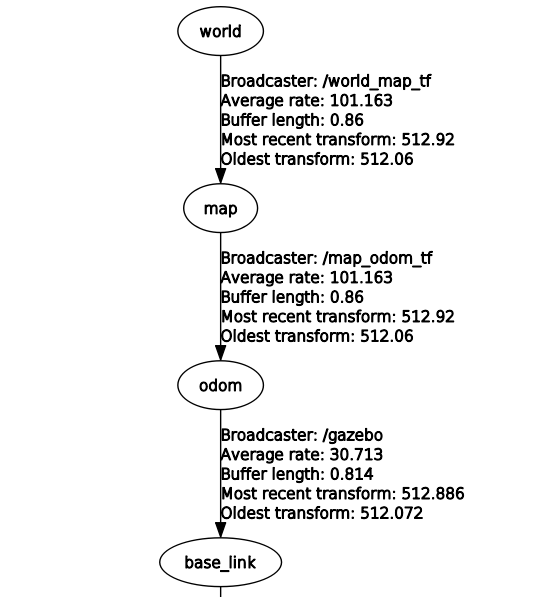
\includegraphics[height=0.6\textheight]{img/velma_tf.png} 
					\caption{początek drzewa transformacji po uruchomieniu symulacji robota}
				\end{center}
			\end{figure}
		\end{column}
	\end{columns}
\end{frame}

\begin{frame}
{Odometria}
	\begin{columns}
		\begin{column}{0.45\textwidth}
			\begin{itemize}
				\item metoda lokalizacji zliczeniowej
				\item obliczenie pozycji robota na podstawie oszacowanej prędkości, kierunku i czasu ruchu
				\item względnie proste zadanie obliczeniowo, ale generuje systematycznie akumulowane błędy
			\end{itemize}
		\end{column}
		\begin{column}{0.55\textwidth}  %%<--- here
			\begin{figure}
				\begin{center}
					\includegraphics[page={180},clip, trim=8cm 1.5cm 3cm 18cm, scale=0.6]{pdf/2017_Book_RoboticsVisionAndControl.pdf}
					\hspace*{15pt}\hbox{\scriptsize{Źródło:\thinspace{\footnotesize{\itshape{Robotics Vision and Control \cite{robotics_vision}}}}}}
					\caption{Błędy odometrii. Niebieska droga oznacza rzeczywistą ścieżkę, czerwona ścieżka obliczoną }
				\end{center}
			\end{figure}
		\end{column}
	\end{columns}
\end{frame}

\begin{frame}
{Lokalizacja z wykorzystaniem znaczników}
	\begin{itemize}
		\item wykorzystuje punkty o znanym położeniu względem początkowego układu współrzędnych mapy, które robot jest w stanie rozróżnić i zidentyfikować
		\item mierząc pozycję robota względem punktów można obliczyć jego pozycję względem początkowego układu mapy
		\item ta metoda również zwraca pozycję z pewnym błędem z powodu niepewności zmierzonej pozycji znaczników, jak i niepewności pomiarowych pozycji ich względem robota, lecz ten błąd jest ograniczony, im lepiej umieszczone znaczniki, tym mniejszy
	\end{itemize}
\end{frame}

\begin{frame}
{Lokalizacja z wykorzystaniem systemu LiDAR}
	\begin{itemize}
		\item problem podobny do poprzedniego, lecz bez rozpoznawania znaczników
		\item wykorzystanie algorytmu ICP (iterative closed point) do dopasowania aktualnego skanu robota do stworzonej uprzednio mapy
		\item niezależność od specjalnych znaczników, lecz większy nakład obliczeniowy
		\item w przypadku gdy zbudowana mapa składa się z podobnych fragmentów może się okazać, że algorytm zawiedzie (przykładowo jazda długim korytarzem bez elementów szczególnych)
	\end{itemize}
\end{frame}



\section{Slam}
\begin{frame}
{Połączenie budowy mapy i lokalizacji}
	\begin{itemize}
		\item W trakcie budowy modelu środowiska często niezbędne jest poruszenie robotem, aby uzyskać wszystkie dane
		\item Poruszenie robota wymaga algorytmu lokalizacji
		\item algorytmy lokalizacji wymagają mapy do minimalizacji błędu uzyskanej pozycji
		\item W celu rozwiązania tego problemu powstał algorytm SLAM (Simulataneous Localization and Mapping)
		\item Zadanie jednoczesnej lokalizacji i budowy mapy trzeba rozwiązywać, gdy mapa środowiska jest niedostępna, a pozycja robota nie jest znana
	\end{itemize}
\end{frame}

\section{Planowanie ścieżki}
\begin{frame}
{Problem planowania ścieżki}
\begin{itemize}
	\item problem popularny również w innych dziedzinach, przykładowo w grach komputerowych \cite{robotics_and_games}
	\item może wykorzystywać standardowe algorytmy przeszukiwania grafu jak A*, Djikstra, zwykle implementowane w zadaniu planowania globalnego
	\item w systemie ROS gotowe do wykorzystania są biblioteki implementujące między innymi algorytmy DWA (Dynamic Window Approach), EBand (elastic band) oraz TEB (Timed Elastic Band), które można wykorzystać do obliczenia pożądanych prędkości bazy mobilnej
\end{itemize}
\end{frame}

\begin{frame}
{Analiza problemu planowania ścieżki}
	Pierwszym punktem jest wybór reprezentacji mapy.
	Szkieletyzacja generuje reprezentację topologiczną środowiska, natomiast dekompozycja komórkowa dzieli przestrzeń wolną od przeszkód na wolne komórki	
	\begin{columns}
		\begin{column}{0.5\textwidth}
			\begin{figure}
				\begin{center}
					\includegraphics[page={3},clip, trim=4cm 15cm 4cm 2cm, scale=0.25]{pdf/A-Comprehensive-Study.pdf}
					\hspace*{5pt}\hbox{\scriptsize{Źródło:\thinspace{\footnotesize{\itshape{Zeyad Abd Algfoor, ... \cite{robotics_and_games}}}}}}
					\caption{Przykłady dekompozycji komórkowej }
				\end{center}
			\end{figure}
		\end{column}
		\begin{column}{0.5\textwidth}  %%<--- here
						\begin{figure}
				\begin{center}
					\includegraphics[page={5},clip, trim=4cm 15cm 4cm 2cm, scale=0.25]{pdf/A-Comprehensive-Study.pdf}
					\hspace*{5pt}\hbox{\scriptsize{Źródło:\thinspace{\footnotesize{\itshape{Zeyad Abd Algfoor, ... \cite{robotics_and_games}}}}}}
					\caption{Przykłady topologii}
				\end{center}
			\end{figure}
		\end{column}
	\end{columns}
\end{frame}

\begin{frame}
{Algorytm generowania ścieżki}
	Po wybraniu odpowiedniej reprezentacji mapy należy zdecydować, który algorytm wyszukiwania drogi zostanie wykorzystany.
	Do algorytmów wspomnianych wcześniej można dodać sztuczne pola potencjału, algorytm genetyczny i wiele innych.
\end{frame}

\begin{frame}
{Istotne szczegóły w kontekście robotyki}
	\begin{itemize}
		\item ścieżka zwykle ma prowadzić od miejsca, w którym znajduje się początkowy układ współrzędnych bazy mobilnej do pozycji sprecyzowanej przez użytkownika
		\item może się okazać, że wyznaczona ścieżka jest zbyt blisko przeszkody i robot w nią uderzy
		\item w celu uniknięcia takich wypadków stosowana jest mapa kosztów i ślad robota (\textit{ang.} footprint)
	\end{itemize}
\end{frame}

\section{Navigation Stack}
\begin{frame}
{ROS Navigation Stack}
	Na następnym slajdzie przedstawione jest podejście do ogólnego problemu nawigacji zaimplementowane i wspierane przez system ROS. 
	Istotnym jest rozdział na część globalną i lokalną.
	Globalna ścieżka wykorzystuje szybkie algorytmy nie zwracające uwagi na przeszkody dynamiczne.
	Lokalny plan generowany na podstawie globalnego jest w stanie na nie reagować.
	Dodatkowo należy zaimplementować system odratowania pozwalający na wyrwanie robota z sytuacji w której planer nie jest w stanie znaleźć drogi do celu.
\end{frame}

\begin{frame}
{Reprezentacja Navigation Stack w systemie ROS}
	\begin{center}
		\begin{figure}
			\centering
			\includegraphics[page={29},clip, trim=0cm 0.5cm 0cm 2cm, scale=0.7]{pdf/Wprowadzenie-do-bloku-robotow-mobilnych.pdf}
			\hspace*{15pt}\hbox{\scriptsize{Źródło:\thinspace{\footnotesize{\itshape{Wojciech Dudek}}}}}
		\end{figure}
	\end{center}
\end{frame}

{
\setbeamertemplate{headline}{}
\addtobeamertemplate{frametitle}{\vspace*{-4\baselineskip}}{}
\begin{frame}
\frametitle{Stan pracy}
	\begin{center}
		\LARGE{\textbf{STAN PRACY}}
	\end{center}
\end{frame}
}

\section{Sformułowanie zadań}
\begin{frame}
{Zadania do wykonania}
Problem ogólny: implementacja systemu nawigacji do symulacji mobilnej bazy wielokierunkowej robota Velma

Założenia:
	\begin{itemize}
		\item budowa mapy na płaskim podłożu i w zamkniętej przestrzeni
		\item mechanizm lokalizacji robota w stworzonym uprzednio środowisku oraz mechanizm jednoczesnej budowy mapy i lokalizacji
		\item mechanizm stworzenia i wykonania ścieżki między dowolnymi dwoma punktami w stworzonym środowisku
	\end{itemize}
\end{frame}




\section{Dotychczasowe wyniki}
\begin{frame}
{Dotychczasowe wyniki pracy}
	\begin{itemize}
		\item naprawa drzewa transformacji
		\item implementacja budowy mapy 3D oraz 2D
		\item implementacja lokalizacji z pomocą czujników LiDAR
		\item uruchomienie planera globalnego wykorzystującego algorytm Dijkstry
		\item uruchomienie planera lokalnego wykorzystującego algorytm DWA oraz TEB
	\end{itemize}
\end{frame}

\section{Zadania do wykonania}
\begin{frame}
{Problem wykrywania przeszkód}
	\begin{itemize}
		\item problem wykrycia blatu stołu
		\item czujniki w bazie mobilnej są w stanie zarejestrować nogi stołu, lecz blatu już nie zauważą
		\item należy wykorzystać kamerę Kinect do wykrycia przeszkód poza zasięgiem czujników LiDAR
		\item istnieje opcja stworzenia oddzielnej mapy kosztów z danych czujników laserowych i oddzielnej z danych kamery Kinect lub połączenia danych w jedną mapę
	\end{itemize}
\end{frame}

\begin{frame}
{Problem algorytmu planowania lokalnego}
	\begin{itemize}
		\item obecnie algorytm planowania lokalnego traktuje bazę jako różnicową, a nie wielokierunkową (holonomiczną)
		\item zostaną przeprowadzone próby dostosowania obecnego planera do możliwości bazy jezdnej
		\item zostaną wyszukane i zaimplementowane inne algorytmy w celu sprawdzenia który jest lepszy
	\end{itemize}
\end{frame}

\begin{frame}
{Przeprowadzanie testów}
	\begin{itemize}
		\item testy z dostępnymi algorytmami lokalizacji, budowy mapy oraz ścieżki
		\item przy lokalizacji sprawdzany będzie błąd względem idealnej pozycji udostępnianiej przez symulator Gazebo
		\item przy planowaniu ścieżki sprawdzany będzie czas wykonania ściezki, reakcja na przeszkody dynamiczne, jakość systemu odratowania i wykorzystanie wszystkich stopni swobody bazy mobilnej
	\end{itemize}
\end{frame}

\section{Zakończenie}
\begin{frame}
	\begin{center}
	\LARGE{\textbf{DZIĘKUJĘ}}
	\end{center}
\end{frame}

%TODO dodaj bibliografię

%\resumenavigation
\end{document}